\section{System Identification}
%TODO: One frequency at a time, cont / discrete
%TODO: several frequencies at once
%TODO: nonparametric methods
%TODO: identifiability
%TODO: LS ausbauen
%TODO: Weightet and recursive least squares
%TODO: Practical aspects

\subsection{Nonparametric Identification}

\subsubsection{One Frequency at a Time}
\begin{minipage}{10cm}
Given an LTI system with a transfer function $G_c(s)$ a sinusoidal 
input signal $u(t) = A \cdot \sin(\omega_0 t)$ will create a sinusoidal
signal $y(t) = B \cdot \sin(\omega_0 t + \varphi) + \text{transient terms}$.
The gain $K = B/A$ can be measured at various frequencies to determine
$G_c(j\omega)$ point-wise.
\end{minipage}
\hspace{0.5cm}
\begin{minipage}{8cm}
    \centering
    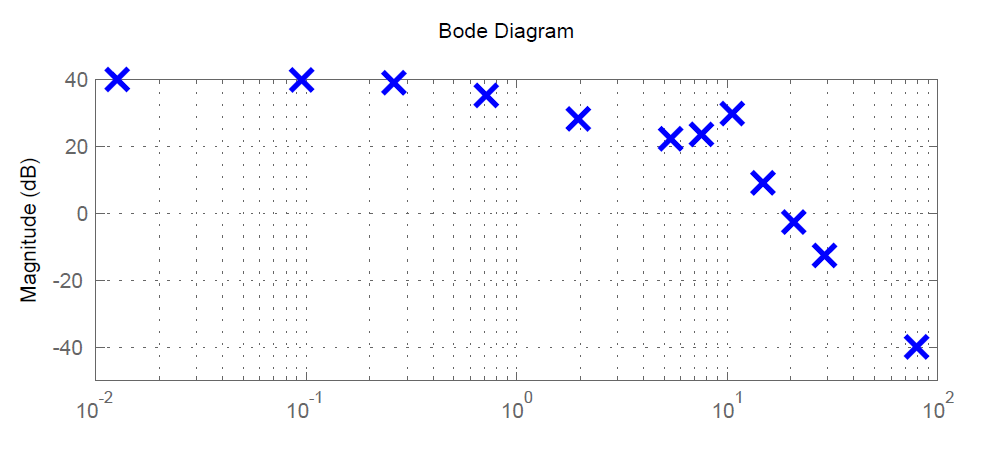
\includegraphics[width=8cm]{bilder/ident_bode.png}
\end{minipage}

\subsubsection{Several Frequencies at Once}

\subsubsection{Further Nonparametric Methods}

\subsection{Parametric Identification}

\subsubsection{Basics of Least Squares (LS)}

$\underbrace{\begin{bmatrix}
	y_2 \\ 
	y_3 \\ 
	\vdots 
\end{bmatrix}}_{y} = 
\underbrace{\begin{bmatrix}
	-y_1 & -y_0 \\ 
	-y_2 & -y_1 \\
	\vdots & \vdots
\end{bmatrix}}_{Y} 
\underbrace{\begin{bmatrix}
	a_1 \\ 
	a_2
\end{bmatrix}}_{a} \longrightarrow a = (Y^TY)^{-1}Y^Ty$

\subsubsection{Weighted Least Squares}

\subsubsection{Recursive Least Squares}

\subsection{Practical Aspects of Identification}